\section{Equations of motion}
In this section the equations of motion for the Cubli are derived in the standard
manipulator equation form and then rewritten in a control affine form.

\subsection{Standard manipulator equation form}
In order to write the equations in the standard manipulator equation form
\begin{equation}
  \label{eq:smform}
  B(\vec{q}) \ddot{\vec{q}} + C(\vec{q}, \dot{\vec{q}}) \dot{\vec{q}} + \vec{G}(\vec{q}) = \vec{Q}
\end{equation}
the inertia matrix $B$, the Coriolis matrix $C$, the gravity term $\vec{G}$ and the generalized forces
$\vec{Q}$ are derived.

\subsubsection{Definition of a configuration vector}
A set of independent generalized coordinates that completely specify the configuration
of the system is given by
\[
\vec{q} =
\begin{bmatrix}
  \theta_{1} & \theta_{2} & \theta_{3} & q_{x} & q_{y} & q_{z}
\end{bmatrix}^T
\]
where the angles $\theta_i$ describe the attitude of the system and
the angles $q_i$ describe the orientation of the flywheels with respect
to the frame of the Cubli.
\par
\begin{figure}[h]
  \centering
  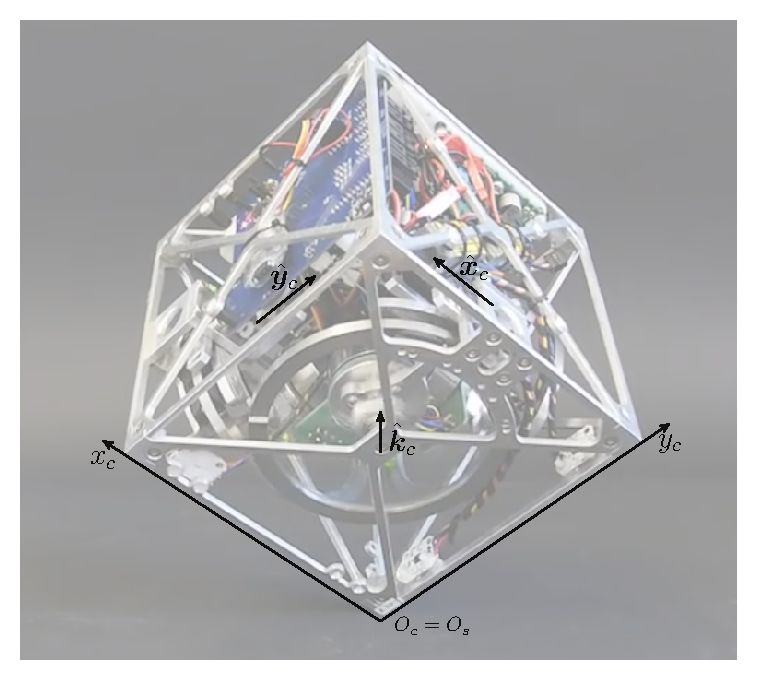
\includegraphics[scale=0.6]{cubli.pdf}
  \caption{Reference frames \label{fig:frames}}
\end{figure}
In order to represent the attitude of the system two reference systems are defined
(see fig. \ref{fig:frames}), a body fixed reference frame
$\{C\} = (O_c; \hat{\vec{i}}_c, \hat{\vec{j}}_c, \hat{\vec{k}}_c)$
and an inertial reference frame $\{S\} = (O_s; \hat{\vec{i}}_s, \hat{\vec{j}}_s, \hat{\vec{k}}_s)$
The attitude of the system is then defined to be the orientation of the frame $\{C\}$
with respect to the frame $\{S\}$ described by the rotation matrix
$R_{SC}$
\[
R_{SC}(\vec{\theta}) = R_z(\theta_1)R_y(\theta_2)R_x(\theta_3)
=
\begin{bmatrix}
  c_1 c_2 & -c_3 s_1 + c_1 s_2 s_3 & c_1 c_3 s_2 + s_1 s_3 \\
  c_2 s_1 & c_1 c_3 + s_1 s_2 s_3 & c_3 s_1 s_2 - c_1 s_3 \\
  -s_2 & c_2 s_3 & c_2 c_3
\end{bmatrix}
\]
where $c_i = \cos{\theta_i}$ and $s_i = \sin{\theta_i}$.

\subsubsection{Derivation of the inertia matrix B}
The inertia matrix B can be derived from the total kinetic energy of the system $T$
\begin{equation}\label{eq:T_general}
  T(\vec{q}, \vec{\dot{q}}) = \frac{1}{2} \dot{\vec{q}}\transpose B(\vec{q}) \dot{\vec{q}}
\end{equation}
In the case of the Cubli the kinetic energy T evaluates to
\begin{equation}\label{eq:T_cubli}
  \begin{split}
    T(\vec{q}, \dot{\vec{q}}) &= \frac{1}{2}(m_c \prescript{c}{}{\vec{v}}_{G_{c}}\transpose \prescript{c}{}{\vec{v}}_{G_{c}} + \prescript{c}{}{\vec{\omega}}_{c}\transpose \prescript{c}{}{\mathfrak{J}}_{G_{c}} \prescript{c}{}{\vec{\omega}}_{c}) \\
    &+ \frac{1}{2}(m_x \prescript{c}{}{\vec{v}}_{G_{x}}\transpose \prescript{c}{}{\vec{v}}_{G_{x}} + \prescript{c}{}{\vec{\omega}}_{x}\transpose \prescript{c}{}{\mathfrak{J}}_{G_{x}} \prescript{c}{}{\vec{\omega}}_{x}) \\
    &+ \frac{1}{2}(m_y \prescript{c}{}{\vec{v}}_{G_{y}}\transpose \prescript{c}{}{\vec{v}}_{G_{y}} + \prescript{c}{}{\vec{\omega}}_{y}\transpose \prescript{c}{}{\mathfrak{J}}_{G_{y}} \prescript{c}{}{\vec{\omega}}_{y}) \\
    &+ \frac{1}{2}(m_z \prescript{c}{}{\vec{v}}_{G_{z}}\transpose \prescript{c}{}{\vec{v}}_{G_{z}} + \prescript{c}{}{\vec{\omega}}_{z}\transpose \prescript{c}{}{\mathfrak{J}}_{G_{z}} \prescript{c}{}{\vec{\omega}}_{z})
  \end{split}
\end{equation}
where $\prescript{c}{}{\vec{v}}_{G_{c}}$ and $\prescript{c}{}{\vec{v}}_{G_{i}}$
are the linear velocities of the centre of mass of the cubic frame and
of the flywheels expressed in $\{C\}$, $\prescript{c}{}{\vec{\omega}}_{c}$
and $\prescript{c}{}{\vec{\omega}}_{i}$ are the angular velocites of the cubic frame
and of the flywheels expressed in $\{C\}$,
$m_c$ and $m_i$ are the mass of the cubic frame and of the flywheels,
$\prescript{c}{}{\mathfrak{J}}_{G_{c}}$ and $\prescript{c}{}{\mathfrak{J}}_{G_{i}}$
are the inertia matrices of the cubic frame and of the flywheels with respect to their
CoMs and expressed in $\{C\}$.
\par
The angular velocity $\prescript{c}{}{\vec{\omega}}_c$ can be expressed as a function of the configuration vector $\vec{q}$
and its derivative $\vec{\dot{q}}$
\[
\prescript{c}{}{\vec{\omega}}_c = \prescript{c}{}{J}_{\omega} (\vec{\theta}) \vec{\dot{q}}
= \prescript{c}{}{J}_{\omega} (\vec{q}) \vec{\dot{q}}
\]
where $\prescript{c}{}{J}_{\omega}(\vec{q})$ is an analytical Jacobian of the form
\begin{equation}\label{eq:ang_cf}
  \prescript{c}{}{J}_{\omega} (\vec{q}) =
  \begin{bmatrix}
    \prescript{c}{}{\tilde{J}}_{\omega} & 0_{3\times3}
  \end{bmatrix} =
  \begin{bmatrix}
    -s_2 & 0 & 1 &\\
    c_2 s_3 & c_3 & 0 & 0_{3\times3}\\
    c_2 c_3 & -s_3 & 0 &
  \end{bmatrix}
\end{equation}
\par
As regards the angular velocites of the flywheels $\prescript{c}{}{\vec{\omega}}_x$,
$\prescript{c}{}{\vec{\omega}}_y$ and $\prescript{c}{}{\vec{\omega}}_z$ the addition theorem
for angular velocites can be used resulting in
\begin{equation}\label{eq:ang_fw}
  \begin{split}
    & \quad \prescript{c}{}{\vec{\omega}}_x = 
    \begin{bmatrix}
      \prescript{c}{}{\tilde{J}_{\omega}} & \vec{e}_1 & \vec{0} & \vec{0}
    \end{bmatrix} \dot{\vec{q}} = \prescript{c}{}{J}_{\omega_{x}} \dot{\vec{q}}\\
    & \quad \prescript{c}{}{\vec{\omega}}_y = 
    \begin{bmatrix}
      \prescript{c}{}{\tilde{J}_{\omega}} & \vec{0} & \vec{e}_2 & \vec{0}
    \end{bmatrix} \dot{\vec{q}} = \prescript{c}{}{J}_{\omega_{y}} \dot{\vec{q}}\\
    & \quad \prescript{c}{}{\vec{\omega}}_z = 
    \begin{bmatrix}
      \prescript{c}{}{\tilde{J}_{\omega}} & \vec{0} & \vec{0} & \vec{e}_3
    \end{bmatrix} \dot{\vec{q}} = \prescript{c}{}{J}_{\omega_{z}} \dot{\vec{q}}
  \end{split}
\end{equation}
\par
The linear velocities $\prescript{c}{}{\vec{v}}_{\vec{G}_{i}}$ can be evaluated using
the well known formula for the velocity of two points fixed on a rigid body
\[
\prescript{c}{}{\vec{v}}_{\vec{G}_{i}} =
\cancelto{0}{\prescript{c}{}{\vec{v}}_{O_{c}}} + \prescript{c}{}{\unitvec{\omega}}_c \prescript{c}{}{\vec{G}}_*
= -\prescript{c}{}{\unitvec{G}}_* \prescript{c}{}{\vec{\omega}}_c
= -\prescript{c}{}{\unitvec{G}}_* \prescript{c}{}{J_{\omega}} \dot{\vec{\theta}}
= -\prescript{c}{}{\unitvec{G}}_* \prescript{c}{}{\tilde{J}_{\omega}} \dot{\vec{q}}
\]
where the position $\vec{G}$ of the CoMs with respect to origin of $\{C\}$ is evaluated with the hypothesis
that the masses of the rigid bodies are distributed uniformly
\[
\prescript{c}{}{\vec{G}}_{c} = 
\begin{bmatrix}
  a/2 \\
  a/2 \\
  a/2
\end{bmatrix} \quad
\prescript{c}{}{\vec{G}}_x = 
\begin{bmatrix}
  0 \\
  a/2 \\
  a/2
\end{bmatrix} \quad
\prescript{c}{}{\vec{G}}_y = 
\begin{bmatrix}
  a/2 \\
  0 \\
  a/2
\end{bmatrix} \quad
\prescript{c}{}{\vec{G}}_z = 
\begin{bmatrix}
  a/2 \\
  a/2 \\
  0
\end{bmatrix} \quad
\]
and the velocity of the point $O_{c}$ evaluates to zero because in
the model considered a spherical joint constraints one of the vertex of the cubic frame from moving.
\par
Finally the inertia matrices of the cubic frame and of the flywheels
evaluate to
\[
\begin{split}
  &\prescript{c}{}{\mathfrak{J}}_{G_{x}} = 
  \begin{bmatrix}
    \frac{m_x r^2}{2} & 0 & 0\\
    0 & \frac{m_x\left(h^2 + 3 r^2 \right)}{12}  & 0\\
    0 & 0 & \frac{m_x\left(h^2 + 3 r^2 \right)}{12}
  \end{bmatrix}
  \quad
  \prescript{c}{}{\mathfrak{J}}_{G_{y}} = 
  \begin{bmatrix}
    \frac{m_y\left(h^2 + 3 r^2 \right)}{12} & 0 & 0\\
    0 & \frac{m_y r^2}{2} & 0\\
    0 & 0 & \frac{m_y\left(h^2 + 3 r^2 \right)}{12}
  \end{bmatrix}\\
  &\prescript{c}{}{\mathfrak{J}}_{G_{z}} = 
  \begin{bmatrix}
    \frac{m_z\left(h^2 + 3 r^2 \right)}{12} & 0 & 0\\
    0 & \frac{m_z\left(h^2 + 3 r^2 \right)}{12} & 0\\
    0 & 0 & \frac{m_z r^2}{2}
  \end{bmatrix}
  \quad
  \prescript{c}{}{\mathfrak{J}}_{G_{c}} = 
  \begin{bmatrix}
    \frac{m_c a^2}{6} & 0 & 0\\
    0 & \frac{m_c a^2}{6} & 0\\
    0 & 0 & \frac{m_c a^2}{6}
  \end{bmatrix}
\end{split}
\]
where $h$ and $r$ are the height and the radius of flywheels respectively.
\par
By inserting all the quantities derived up to now in the equation (\ref{eq:T_cubli})
and using the more general form of $T$ given in equation (\ref{eq:T_general}) the inertia
matrix B is obtained
\[
\begin{split}
  B(\vec{q}) &= m_c \prescript{c}{}{J}_{\omega}\transpose \prescript{c}{}{\unitvec{G}}_{c} \transpose  \prescript{c}{}{\unitvec{G}}_{c} \prescript{c}{}{J}_{\omega} + \prescript{c}{}{J}_{\omega}\transpose  \prescript{c}{}{\mathfrak{J}}_{G_{c}} \prescript{c}{}{J}_{\omega} \\
  &+ m_x \prescript{c}{}{J}_{\omega}\transpose \prescript{c}{}{\unitvec{G}}_{x} \transpose  \prescript{c}{}{\unitvec{G}}_{x} \prescript{c}{}{J}_{\omega} + \prescript{c}{}{J}_{\omega_{x}}\transpose  \prescript{c}{}{\mathfrak{J}}_{G_{x}} \prescript{c}{}{J}_{\omega_{x}} \\
  &+ m_y \prescript{c}{}{J}_{\omega}\transpose \prescript{c}{}{\unitvec{G}}_{y} \transpose  \prescript{c}{}{\unitvec{G}}_{y} \prescript{c}{}{J}_{\omega} + \prescript{c}{}{J}_{\omega_{y}}\transpose  \prescript{c}{}{\mathfrak{J}}_{G_{y}} \prescript{c}{}{J}_{\omega_{y}} \\
  &+ m_z \prescript{c}{}{J}_{\omega}\transpose \prescript{c}{}{\unitvec{G}}_{z} \transpose  \prescript{c}{}{\unitvec{G}}_{z} \prescript{c}{}{J}_{\omega} + \prescript{c}{}{J}_{\omega_{z}}\transpose  \prescript{c}{}{\mathfrak{J}}_{G_{z}} \prescript{c}{}{J}_{\omega_{z}} \\
\end{split}
\]

Since the jacobians $\prescript{c}{}{J}_{\omega}$,
$\prescript{c}{}{J}_{\omega_{x}}$,
$\prescript{c}{}{J}_{\omega_{y}}$,
$\prescript{c}{}{J}_{\omega_{z}}$
only depends on the angles $\theta_2$ and $\theta_3$
and the other quantities appearing in the inertia matrix
are constant then
\[
B(\vec{q}) = B(\theta_2, \theta_3)
\]
This fact is a consequence of the form of the analytical jacobian
$\prescript{c}{}{\tilde{J}}_{\omega}$ and does not depend on the particular Euler parametrization chosen.

\subsubsection{Derivation of the Coriolis matrix C}
The Coriolis matrix C can be written as
\[
C_{ij} = \sum_{k=1}^6{\Gamma^i_{jk} \dot{q}_k}
\]
where $\Gamma^i_{jk}$ are the Christoffel Symbol of the First Kind
\[
\Gamma^i_{jk} = \frac{1}{2} \left ( \frac{\partial B_{ij}}{\partial q_k}
+ \frac{\partial B_{ik}}{\partial q_j}
- \frac{\partial B_{jk}}{\partial q_i}\right)
\]

\subsubsection{Derivation of the gravity term $\vec{G}$}
The gravity term $\vec{G}$ can be evaluated as
\[
\vec{G} =\left(\frac{\partial U}{\partial \vec{q}}\right) \transpose
\]
where $U$ is the total potential energy of the system given by
\[
U(\vec{q}) = - \prescript{c}{}{\vec{g}} \transpose
(m_c  \prescript{c}{}{\vec{G}}_c +
m_x  \prescript{c}{}{\vec{G}}_x +
m_y  \prescript{c}{}{\vec{G}}_y +
m_z  \prescript{c}{}{\vec{G}}_z)
\]
and the gravitational acceleration vector $\prescript{c}{}{\vec{g}}$ can be obtained as
\[
\prescript{c}{}{\vec{g}} = R_{SC}\transpose \prescript{s}{}{\vec{g}} = R_{SC}\transpose 
\begin{bmatrix}
  0\\
  0\\
  -g
\end{bmatrix}
\]

\subsubsection{Derivation of the generalized forces $\vec{Q}$}
The $i$-th generalized force $Q_i$ for the Cubli evaluates to
\[
\begin{split}
  Q_i = & \tau_{x} \hat{\vec{i}}_c^{T} \frac{\partial (\prescript{c}{}{\vec{\omega}_x})}{\partial \dot{q}_i} +
  \tau_{y} \hat{\vec{j}}_c^{T} \frac{\partial (\prescript{c}{}{\vec{\omega}_y})}{\partial \dot{q}_i} +
  \tau_{z} \hat{\vec{k}}_c^{T} \frac{\partial (\prescript{c}{}{\vec{\omega}_z})}{\partial \dot{q}_i} -\\
  &\left( \tau_{x} \hat{\vec{i}}_c^{T} \frac{\partial (\prescript{c}{}{\vec{\omega}_c})}{\partial \dot{q}_i} +
  \tau_{y} \hat{\vec{j}}_c^{T} \frac{\partial (\prescript{c}{}{\vec{\omega}_c})}{\partial \dot{q}_i} +
  \tau_{z} \hat{\vec{k}}_c^{T} \frac{\partial (\prescript{c}{}{\vec{\omega}_c})}{\partial \dot{q}_i}\right)
\end{split}
\]
where $\tau_x$, $\tau_y$ and $\tau_z$ are the torques applied to the flywheels and
$-\tau_x$, $-\tau_y$ and $-\tau_z$ are the torques applied to the cubic frame.
\par
By using the Jacobians defined in equations (\ref{eq:ang_cf}) and (\ref{eq:ang_fw})
the expression becomes
%% \prescript{c}{}{J}_{\omega_{x}} 
\[
\begin{split}
  Q_i = & \tau_{x} \hat{\vec{i}}_c^{T} \prescript{c}{}{J}_{\omega_{x}}(:,i)+
  \tau_{y} \hat{\vec{j}}_c^{T} \prescript{c}{}{J}_{\omega_{y}}(:,i)+
  \tau_{z} \hat{\vec{k}}_c^{T} \prescript{c}{}{J}_{\omega_{z}}(:,i) -\\
  &( \tau_{x} \hat{\vec{i}}_c  +
  \tau_{y} \hat{\vec{j}}_c  +
  \tau_{z} \hat{\vec{k}}_c )^{T} \prescript{c}{}{J}_{\omega}(:,i)
\end{split}
\]
Since the columns of the Jacobians are the same
\[
\prescript{c}{}{J}_{\omega_{x}}(:,i) =
\prescript{c}{}{J}_{\omega_{y}}(:,i) =
\prescript{c}{}{J}_{\omega_{z}}(:,i) =
\prescript{c}{}{J}_{\omega}(:,i) =
\prescript{c}{}{\tilde{J}}_{\omega}(:,i)
\]
for $i = 1, 2, 3$ then
\[
Q_i = (\tau_{x} \hat{\vec{i}}_c  +
\tau_{y} \hat{\vec{j}}_c  +
\tau_{z} \hat{\vec{k}}_c  -
\tau_{x} \hat{\vec{i}}_c  -
\tau_{y} \hat{\vec{j}}_c  -
\tau_{z} \hat{\vec{k}}_c)^{T} \prescript{c}{}{\tilde{J}}_{\omega}(:,i) = 0
\]
As regards the other indexes
\[
\prescript{c}{}{J}_{\omega_{x}}(:,i + 3) =
\prescript{c}{}{J}_{\omega_{y}}(:,i + 3) =
\prescript{c}{}{J}_{\omega_{z}}(:,i + 3) =
\vec{e}_i
\quad
\prescript{c}{}{J}_{\omega}(:,i + 3) = \vec{0}
\]
for $i = 1, 2, 3$ resulting in
\[
Q_4 = \tau_{x} \hat{\vec{i}}_c^{T} \vec{e}_1 +
\tau_{y} \hat{\vec{j}}_c^{T} \vec{e}_1 + 
\tau_{z} \hat{\vec{k}}_c^{T} \vec{e}_1 -
( \tau_{x} \hat{\vec{i}}_c  +
\tau_{y} \hat{\vec{j}}_c  +
\tau_{z} \hat{\vec{k}}_c )^{T} \vec{0} = \tau_{x} \vec{e}_{1}^{T} \vec{e}_1
= \tau_{x}
\]
\[
Q_5 = \tau_{x} \hat{\vec{i}}_c^{T} \vec{e}_2 +
\tau_{y} \hat{\vec{j}}_c^{T} \vec{e}_2 + 
\tau_{z} \hat{\vec{k}}_c^{T} \vec{e}_2 -
( \tau_{x} \hat{\vec{i}}_c  +
\tau_{y} \hat{\vec{j}}_c  +
\tau_{z} \hat{\vec{k}}_c )^{T} \vec{0} = \tau_{y} \vec{e}_{2}^{T} \vec{e}_2
= \tau_{y}
\]
\[
Q_6 = \tau_{x} \hat{\vec{i}}_c^{T} \vec{e}_3 +
\tau_{y} \hat{\vec{j}}_c^{T} \vec{e}_3 + 
\tau_{z} \hat{\vec{k}}_c^{T} \vec{e}_3 -
( \tau_{x} \hat{\vec{i}}_c  +
\tau_{y} \hat{\vec{j}}_c  +
\tau_{z} \hat{\vec{k}}_c )^{T} \vec{0} = \tau_{z} \vec{e}_{3}^{T} \vec{e}_3
= \tau_{z}
\]
The resulting vector of generalized forces is
\[
\vec{Q} =
\begin{bmatrix}
  0 & 0 & 0 & \tau_x & \tau_y & \tau_z
\end{bmatrix}^{T} = 
\begin{bmatrix}
  0 & 0 & 0 & \vec{\tau}
\end{bmatrix}^{T}
= F \vec{\tau}
\]
where
\[
F =
\begin{bmatrix}
  0_{3\times3} \\
  I_{3\times3}
\end{bmatrix}
\]
has rank $3 < 6$ for every configuration resulting in a underactuated system.

\subsection{Equations in control affine form}
The equation (\ref{eq:smform}) in standard manipulator form can be written in a control affine
form for control purposes with the following procedure.
\par
First a new state $\tilde{x}$ for the system is defined
\[
\tilde{\vec{x}} =
\begin{bmatrix}
  \vec{x}_1 \\
  \vec{x}_2
\end{bmatrix} = 
\begin{bmatrix}
  \vec{q} \\
  \vec{\dot{q}}
\end{bmatrix}
\]
The time rate of change of the state can then be written using (\ref{eq:smform})
\begin{equation}\label{eq:nl_eq_1}
  \begin{split}
    \dot{\tilde{\vec{x}}} =
    \begin{bmatrix}
      \dot{\tilde{\vec{x}}}_1 \\
      \dot{\tilde{\vec{x}}}_2
    \end{bmatrix} &= 
    \begin{bmatrix}
      \tilde{\vec{x}}_2 \\
      - B({\tilde{\vec{x}}_1}) ^ {-1} (C(\tilde{\vec{x}}_1, \tilde{\vec{x}}_2) \tilde{\vec{x}}_2 + \vec{G}(\tilde{\vec{x}}_1)) 
    \end{bmatrix} +
    \begin{bmatrix}
      \vec{0} \\
      B({\tilde{\vec{x}}_1}) ^ {-1} \vec{Q}
    \end{bmatrix}\\
    &=\begin{bmatrix}
    \tilde{\vec{x}}_2 \\
    - B^ {-1} (C \tilde{\vec{x}}_2 + \vec{G}) 
    \end{bmatrix} +
    \begin{bmatrix}
      0_{6\times3} \\
      B({\tilde{\vec{x}}_1}) ^ {-1} F
    \end{bmatrix}\vec{\tau}\\
        &=\begin{bmatrix}
    \tilde{\vec{x}}_2 \\
    - B^ {-1} (C \tilde{\vec{x}}_2 + \vec{G}) 
    \end{bmatrix} +
    \begin{bmatrix}
      0_{6\times3} \\
      \left(B({\tilde{\vec{x}}_1}) ^ {-1}\right)_{(:, 4:6)}
    \end{bmatrix}\vec{\tau}\\
    &= \tilde{\vec{f}}(\tilde{\vec{x}}) + \tilde{g}(\tilde{\vec{x}}) \vec{\tau}\\
    &= \tilde{\vec{f}}(\tilde{\vec{x}}) + \tilde{g}(\tilde{\vec{x}}) \vec{u}
  \end{split}
\end{equation}
thus obtaining a control affine form of the equations.
\par
It can be verified that $B$, $C$ and $\vec{G}$ does not depend on the angular position of the flywheels.
Since the position of the flywheels is of no interest for control purposes the $4$-th, $5$-th and $6$-th rows
of (\ref{eq:nl_eq_1}) can be neglected and the state can be reduced to
\[
\begin{split}
  \vec{x} &=
  \begin{bmatrix}
    \theta_1 & \theta_2 & \theta_3 & \dot{\theta}_1 & \dot{\theta}_2 & \dot{\theta}_3 & \dot{q}_x & \dot{q}_y & \dot{q}_z
  \end{bmatrix}\transpose\\
  &=\begin{bmatrix}
  \vec{\theta} & \vec{\dot{\theta}} & \vec{\dot{q}}_{wheels}
  \end{bmatrix}\transpose
\end{split}
\]
The time rate of change of the state updates to
\begin{equation}\label{eq:nl_eq_2}
  \dot{\vec{x}} = \vec{f}(\vec{x}) + g(\vec{x}) \vec{u}
\end{equation}
where $\vec{f}$ and $g$ are obtained from $\tilde{\vec{f}}$ and
$\tilde{g}$ by removing the $4$-th, $5$-th and $6$-th rows.
\par
The outputs of the system are chosen as
\begin{equation}\label{eq:output}
\vec{y} = \vec{h}(\vec{x}) =
\begin{bmatrix}
  \theta_1 &
  \theta_2 &
  \theta_3
\end{bmatrix}^T
\end{equation}

\subsection{Equlibrium points}
Among the many equilibria of the system (\ref{eq:nl_eq_2}) the sets
\begin{small}
  \[
  \mathcal{E}_{1} = \left\{ \vec{x} \mid \theta_1 \in [-\pi, \pi),\enspace \theta_2 = -\mathrm{atan}\frac{\sqrt{2}}{2},\enspace
    \theta_3 = \frac{\pi}{4},\enspace
    \vec{\dot{\theta}} = \vec{0},\enspace
    \vec{\dot{q}}_{wheels} = \vec{0},\enspace
    \vec{u} = \vec{0}
    \right\}
    \]
\end{small}
\begin{small}
  \[
  \mathcal{E}_{2} = \left\{
  \vec{x} \mid \theta_1 \in [-\pi, \pi),\enspace
    \theta_2 = \mathrm{atan}\frac{\sqrt{2}}{2},\enspace
    \theta_3 = -\frac{3}{4} \pi,\enspace
    \vec{\dot{\theta}} = \vec{0},\enspace
      \vec{\dot{q}}_{wheels} = \vec{0},\enspace
      \vec{u} = \vec{0}
      \right\}
      \]
\end{small}
are of interest. The set $\mathcal{E}_{1}$ is that of the upright
equilibria which is unstable and the set $\mathcal{E}_{2}$ is of that
of the hanging equilibria which is stable in the sense of Laypunov.
\par
The values of the angles $\theta_1$, $\theta_2$ and
$\theta_3$ can be easily found from the geometry of the cubic frame (see fig \ref{fig:cubli_equilibria}).
\begin{figure}[h]
  \centering
  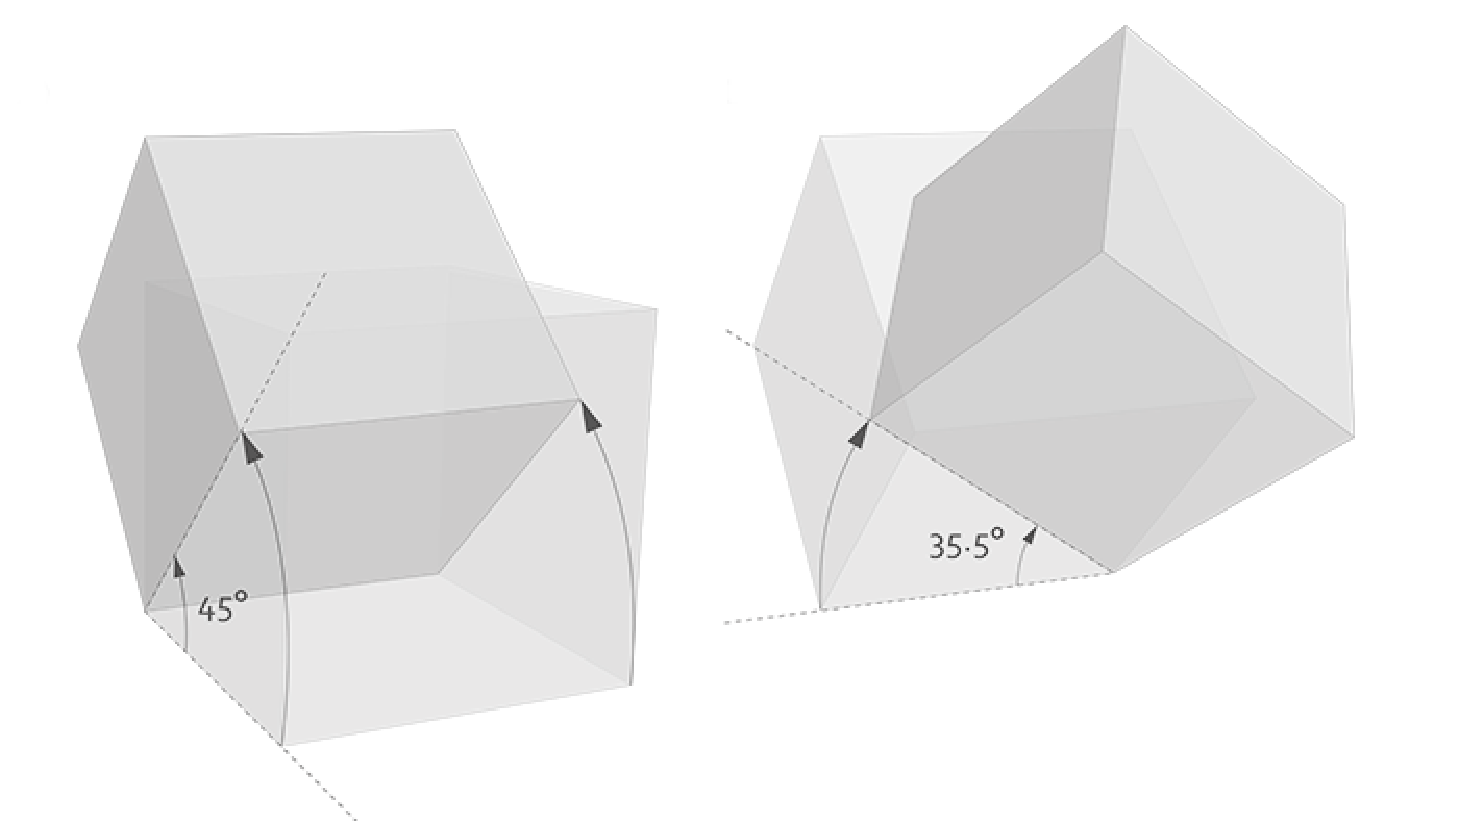
\includegraphics[scale=0.5]{cubli_equilibria}
  \caption{Upright equilibium configuration of the Cubli\label{fig:cubli_equilibria}}
\end{figure}
In particular the angle $\theta_1$ clearly represents the yaw of the cubic
frame in the upright or hanging position.
\par
It should be noted that other equilibria exist in which the system is
at rest in the upright or hanging position while the flywheels rotates
at a non zero constant angular velocity.

\subsection{Parameters of the system}
In the rest of this report the following values are used for the parameters of the system
\begin{itemize}
  \item[-] $M = \SI{2.5}{kg}$;
  \item[-] $m = \SI{0.204}{kg}$;
  \item[-] $a = \SI{0.15}{m}$;
  \item[-] $r = \SI{0.05}{m}$;
  \item[-] $h = \SI{0.005}{m}$;
\end{itemize}
\newpage
